\documentclass{standalone}
\usepackage{mathrsfs}
\usepackage[x11names]{xcolor}
\usepackage{tikz, tkz-euclide}
%\usepackage[american]{circuitikz}
\usepackage{siunitx}
\usepackage{textcomp}
\usetikzlibrary{arrows}
\begin{document}

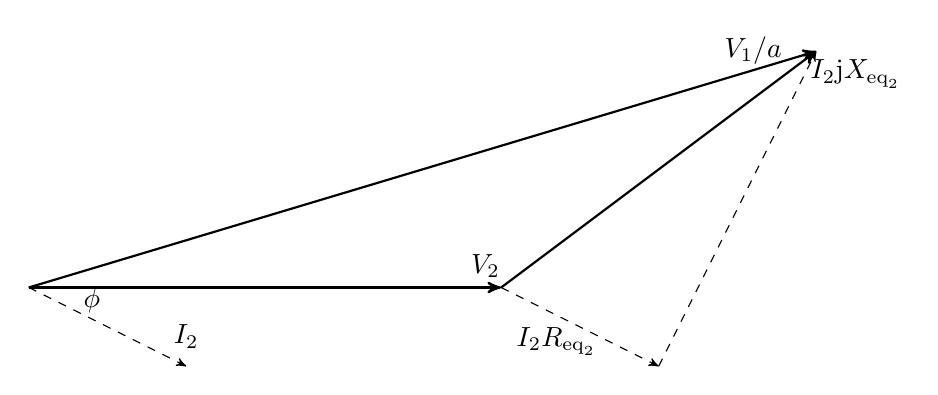
\begin{tikzpicture}[draw=black,thick]
\draw[->,>=stealth'] (0,0) -- (6,0);
\draw[->,>=stealth',thin,dashed] (0,0) -- (2,-1);
\draw[->,>=stealth',thin,dashed] (6,0) -- (8,-1);
\draw[->,>=stealth',thin,dashed] (8,-1) -- (10,3);
\draw[->,>=stealth'] (6,0) -- (10,3);
\draw[->,>=stealth'] (0,0) -- (10,3);
\tkzLabelPoint[above](0.8,-0.45){{\(\phi\)}}
\tkzLabelPoint[above](2,-0.9){{\(I_{2}\)}}
\tkzLabelPoint[above](5.8,0){{\(V_{2}\)}}
\tkzLabelPoint[above](6.7,-1){{\(I_{2}R_{\mathrm{eq}_{2}}\)}}
\tkzLabelPoint[above](10.5,2.4){{\(I_{2}\mathrm{j}X_{\mathrm{eq}_{2}}\)}}
\tkzLabelPoint[above](9.2,2.7){{\(V_{1}/a\)}}

\end{tikzpicture}
\end{document}
